
\documentclass[t, 11pt]{beamer}
%\pdfmapfile{+sansmathaccent.map}
%%% Работа с русским языком
\usepackage{cmap}				
\usepackage{mathtext} 				
\usepackage[T2A]{fontenc}		
\usepackage[utf8]{inputenc}			
\usepackage[russian, english]{babel}	

\usetheme{Montpellier}
\usecolortheme{beaver} % Цветовая схема

\usepackage{advdate}



%%% Работа с картинками
\usepackage{graphicx}

\usepackage{csquotes}

\hypersetup{				
	colorlinks=true,       	
	linkcolor=blue,          
	citecolor=black,       
	filecolor=magenta,      
	urlcolor=red           
}
%% табличка
\usepackage{booktabs, caption, makecell}
\usepackage{threeparttable}

%% график нормального распределения 
\usepackage{tikz}
\usepackage{xcolor}
\usepackage{pgfplots}
\pgfplotsset{compat=1.7}

%% доп символы
\usepackage{newunicodechar}

\newcommand\Warning{%
	\makebox[1.4em][c]{%
		\makebox[0pt][c]{\raisebox{.1em}{\small!}}%
		\makebox[0pt][c]{\color{red}\Large$\bigtriangleup$}}}%

%\newunicodechar{⚠}{\Warning}

\title {Diagnostics}
\subtitle{How to deal with linear regression}
\author{Chuvakin Sergey}
\date{\AdvanceDate[+1]\today}
\institute[<<Anthropology and Sociology major>>]{<<School of Advanced Studies>>}

\begin{document}
	
	
	\frame[plain]{\titlepage}		
	
	\section{Outline}
	
	\begin{frame} 
		\frametitle{\insertsection} 
		\begin{itemize}
			\item Why?
			\item Efficient Sample
			\item Multicollinearity
			\item Linear dependency 
			\item Homoscedasticity
			\item Exogeneity
			\item Model Selection
		\end{itemize}
		
	\end{frame}



\section{why}	
\begin{frame} 
		\frametitle{\insertsection} 
			Diagnosticts helps to understand if regression model is efficient,  robust and unbiased. 
			We can use and interpret just in case our coefficients are unbaised.
		
	\end{frame}
	
\section{Efficient Sample}
\begin{frame} 
	\frametitle{\insertsection} 
		Sample is implied to be representative. First of all it assumed to be random, but in case other technique is chosen, it should be proven. 
	
\end{frame}


%% https://dspace.mit.edu/bitstream/handle/1721.1/48530/multicollinearit00farr.pdf?sequence=1	
	\section{Multicollinearity}
	\begin{frame} 
		\frametitle{\insertsection} 
		\begin{itemize}
		\item Collinearity is a linear association between two explanatory variables
		\item Multicollinearity refers to a situation in which two or more explanatory variables in a multiple regression model are highly correlated with each other
		\item 	For more information click \href{https://dspace.mit.edu/bitstream/handle/1721.1/48530/multicollinearit00farr.pdf?sequence=1	}{here}
		\end{itemize}
	
	You can also use Variance Inflation Factor (VIF).
		$$
		VIF  = \frac{1}{1 - R^2_j}
		$$
	where $R^2_j$ is the coefficient of determination of a regression of explanatory variable j on all the other explanatory variables.
	
	VIF should be less than 4.
	\end{frame}

\begin{frame} 
	\frametitle{\insertsection}
	 \begin{center}
		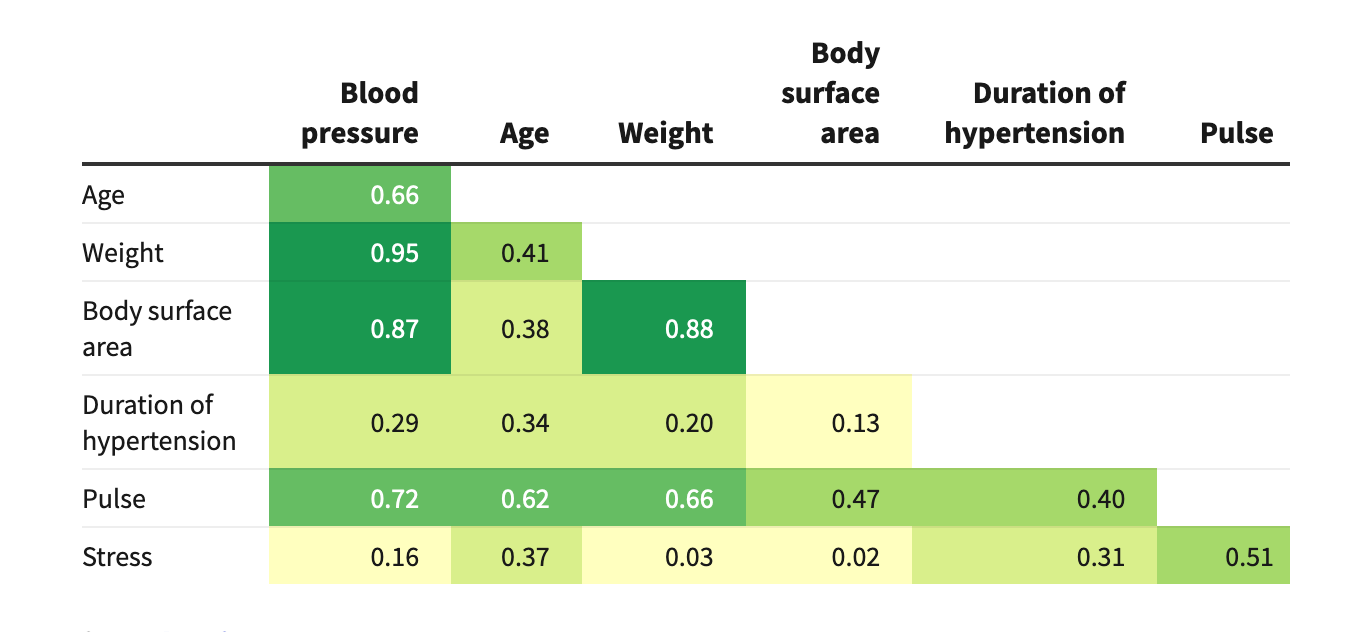
\includegraphics[scale=0.4]{multicol1}
	\end{center}
\end{frame}	

	\section{Linear dependency}
\begin{frame} 
	\frametitle{\insertsection} 
	 By default true relationship should resamble linear. Make scatter plot to ensure it. But, unfortunately, there is a really little chance that you face it. In these cases use some function to transform your X in regression formula. For example add a quadratic (second-order) polynomial of X if you see a U-shape relationship between Y and X (cubic, or third-order, if a Sigma-shape link). You can use any function are known, the only condition - is should satisfy visual relationship. 
\end{frame}	

	\section{Homoscedasticity}
\begin{frame} 
	\frametitle{\insertsection} 
	 \begin{center}
	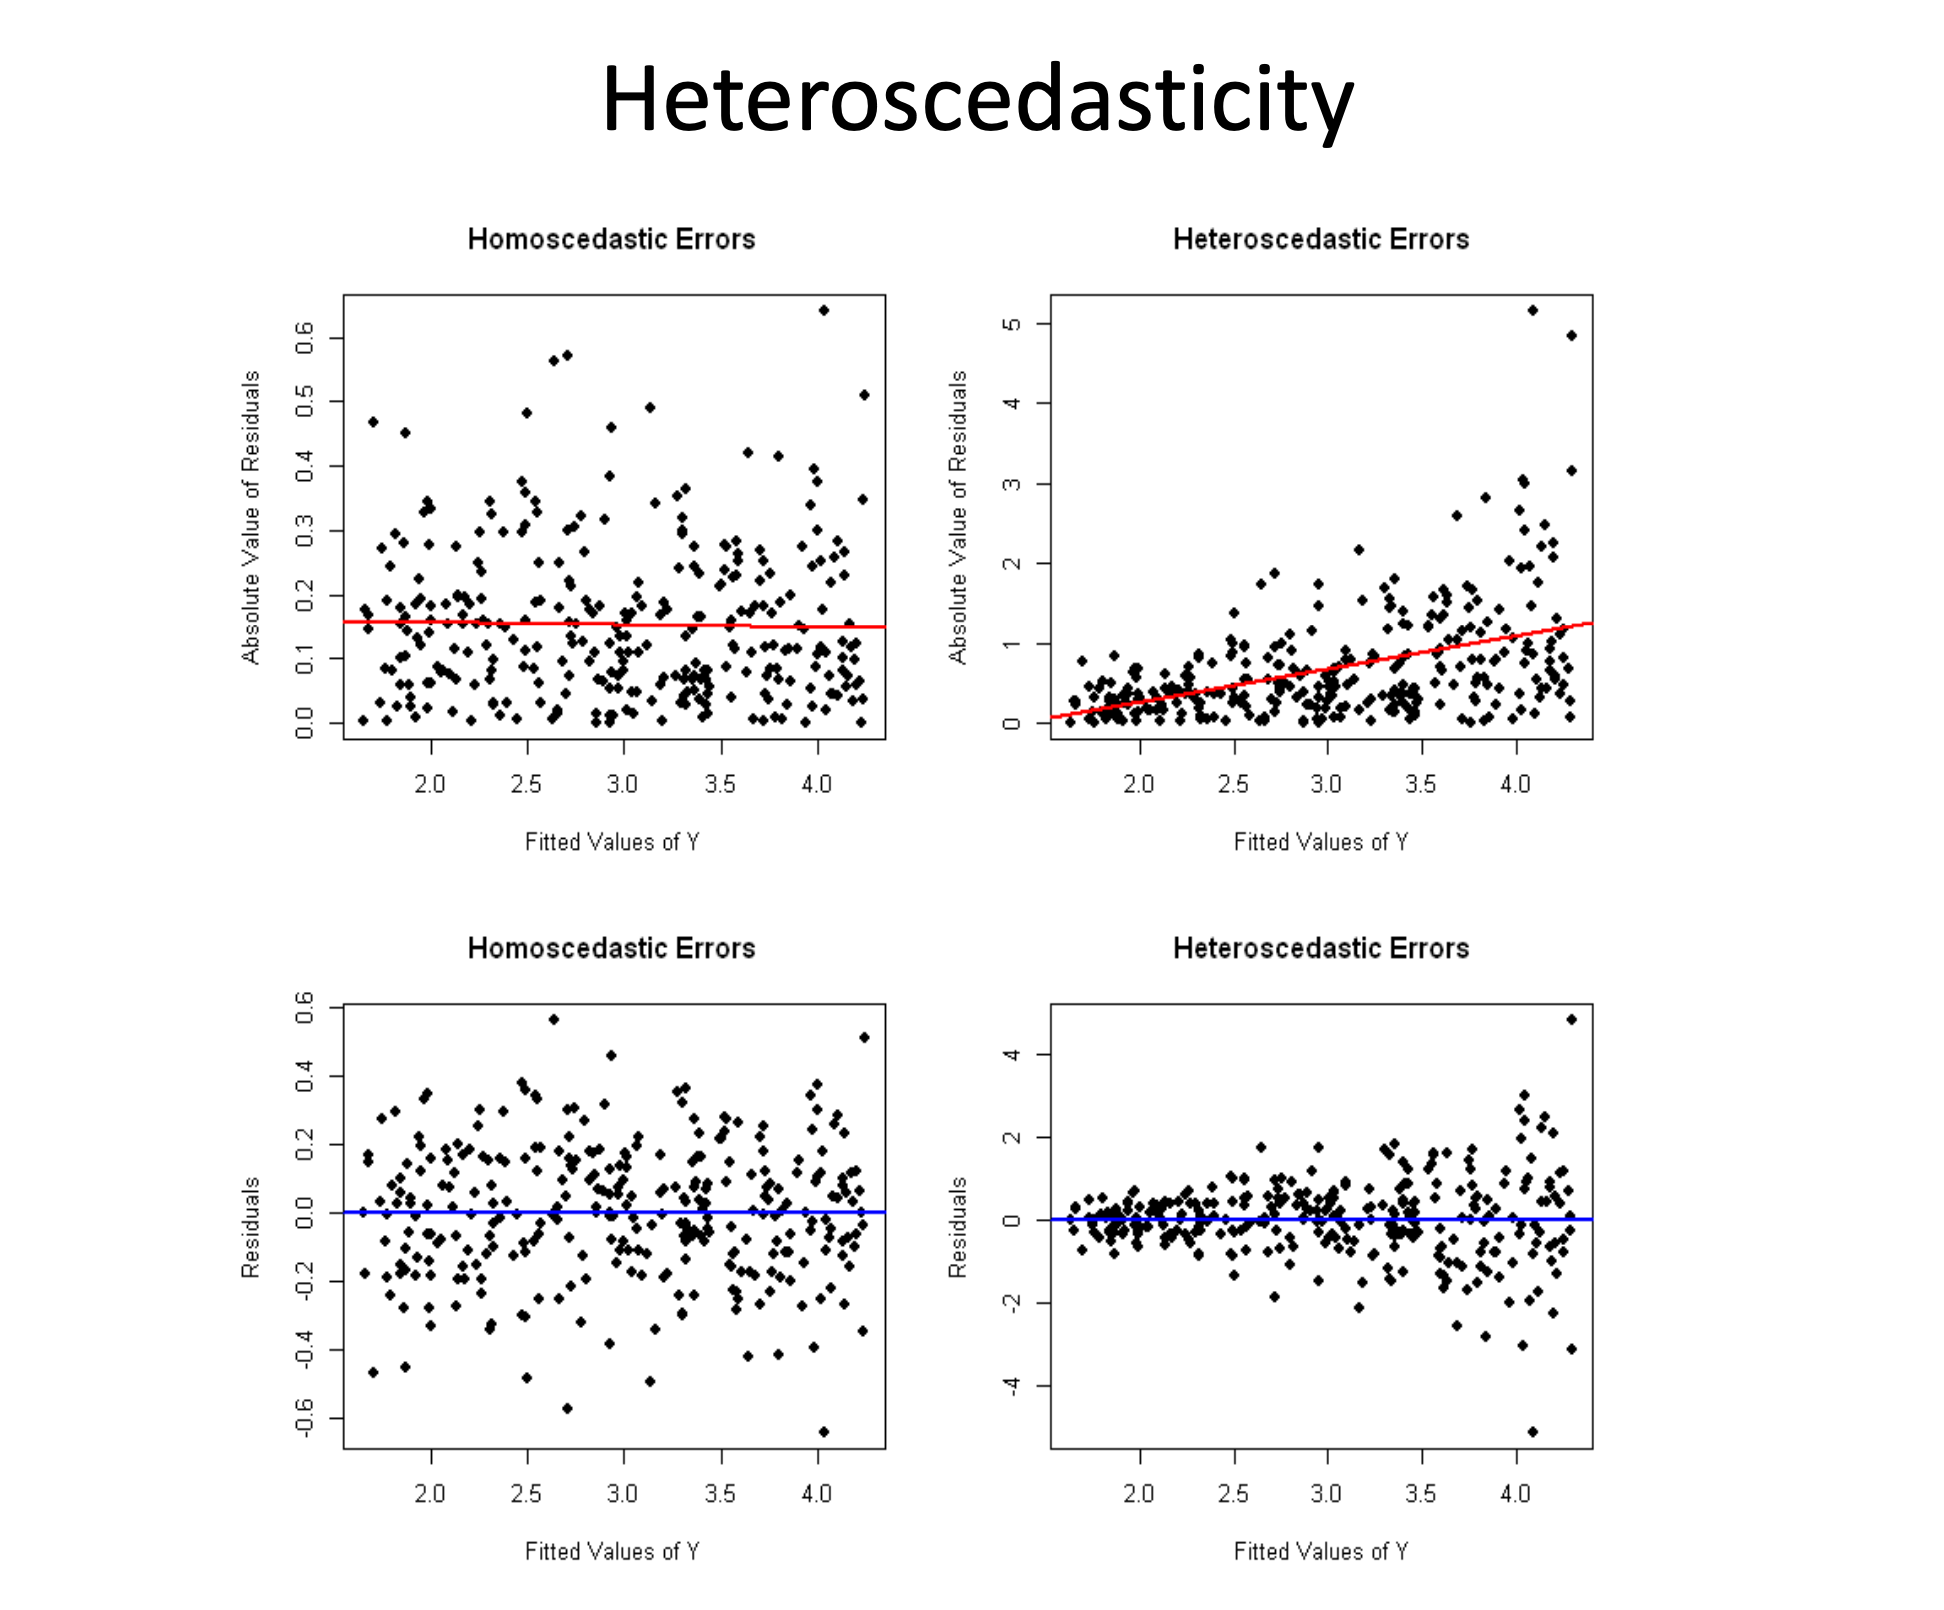
\includegraphics[scale=0.25]{hetero}
\end{center}
\end{frame}	

\begin{frame} 
	\frametitle{\insertsection} 
	\begin{itemize}
 		\item The term <<heteroscedasticity>> refers to the case of non-constant error variance. 
 		\item Standard errors obtained under heteroskedastictity are generally incorrect
 	\end{itemize}
	 Except for visually representativness it also could be captured via Breusch-Pagan test. In R, this test can be performed by the function ncvTest from the car package or the function bptest from the lmtest package. Significant tests indicate heteroskedastisity. Use p-values to decide. 
\end{frame}	

	\section{Exogeneity}
\begin{frame} 
	\frametitle{\insertsection} 
	
	\begin{itemize}
		\item Exogeneity means that each X variable does not depend on the dependent variable Y, ratherY depends on theXs and on e
		\item Since Y depends on e, this means that the Xs are assumed to be independent of Y hence e
		\item required because if the <<independent variables>> are not independent of e and Y, then the estimated regression coefficients are not consistentif we use the OLS estimating equations
		
		\item X is exogenous if $Corr(X, e) = 0$
		\item X is endogenous if $Corr(X, e) \neq 0$
		\item If OLS is to be unbiased and consistent, requires that X is exogenous.
	\end{itemize}
	
\end{frame}	

\begin{frame} 
	\frametitle{\insertsection} 
	
	\begin{itemize}
		\item Simultaneous equations bias
		\item Omitted variables bias
		\item Errors-in-variables
		\item Regression model (time series) includes a lagged dependent variable and the error term is serially correlated.
	\end{itemize}
	
\end{frame}	

	\section{Model Selection}
\begin{frame} 
	\frametitle{\insertsection} 
	How to choose model between several?
	\begin{itemize}
		\item $R^2$ should be close to 1 
		\item AIC – Akaike Information Criterion, should be less
		\item BIC – Bayesian Information Criterion, should be less
		\end{itemize}
\end{frame}	

\section{What else?}
\begin{frame} 
	\frametitle{\insertsection} 
	\begin{itemize}
		\item Think about standartization
		\item Remove extreme values
	\end{itemize}
\end{frame}	
	
\end{document}